% Tento soubor nahraďte vlastním souborem s přílohami (nadpisy níže jsou pouze pro příklad)
% This file should be replaced with your file with an appendices (headings below are examples only)

% Umístění obsahu paměťového média do příloh je vhodné konzultovat s vedoucím
% Placing of table of contents of the memory media here should be consulted with a supervisor
\chapter{Obsah přiloženého paměťového média}

\begin{itemize}
    \item \texttt{install} -- Obsahuje instalační skript knihovny \texttt{OpenCV 3.4.2}.
    \item \texttt{src} -- Zdrojové kódy generátoru datových sad (\texttt{Datagen}) a použité neuronové sítě (\texttt{Darknet}).
    \item \texttt{utils} -- Skripty a programy (vytvořené či volně dostupné) používané v průběhu práce, zejména ke konverzi formátů anotací a~k~vyhodnocení.
    \item \texttt{doc} -- Programová dokumentace a plakát použitý k prezentaci této práce.
    \item \texttt{README} -- Více obsáhlá příručka v~anglickém jazyce (ve formátu \texttt{.md} -- \emph{markdown}, i~s~přiloženými obrázky).
    \item \texttt{videos} -- Video prezentující dosažené výsledky.
    \item \texttt{report} -- Adresář obsahující zdrojové kódy tohoto dokumentu ve formátu \LaTeX, a~také jejich přeloženou verzi ve formátu PDF.
\end{itemize}


\chapter{Manuál}

Sestavení a použití generátoru datových sad \texttt{Datagen} na linuxovém OS:

\begin{enumerate}
    \item Instalace \texttt{OpenCV} pomocí přiloženého instalačního skriptu příkazem\\ \texttt{bash install/install-opencv.sh} v kořenovém adresáři projektu.
    \item Umístit obrázky pozadí do adresáře \texttt{data/backgrounds} (již obsahuje několik příkladů).
    \item Umístit snímky značek do adresářů \texttt{data/cropped} a \texttt{data/transparent}. Každá třída značek má svůj vlastní pod-adresář a v ní soubor \texttt{imgClass} obsahující pouze název třídy (již obsahuje několik příkladů).
    \item Nastavení konstant v \texttt{Makefile} (výběr efektů a způsobu generování).
    \item Spuštění kompilace pomocí napsání příkazu \texttt{make} v kořenovém adresáři projektu.
    \item Po úspěšné kompilaci -- spuštění generování pomocí již vytvořených cílů v \texttt{Makefile}:
    \begin{itemize}
        \item V případě ořezaných značek: \texttt{make runc}.
        \item V případě transparentních značek: \texttt{make runt}.
    \end{itemize}
    \item Vytvořená datová sada by se měla nacházet v adresáři \texttt{out}.
\end{enumerate}
Sestavení a použití neuronové sítě \texttt{Darknet} na linuxovém OS:

\begin{enumerate}
    \item Nastavení kompilačních konstant v \texttt{Makefile}. Před-nastaveno tak, jak bylo používáno v této práci.
    \item Kompilace pomocí příkazu \texttt{make} v kořenovém adresáři projektu.
    \item Nastavení konfiguračního souboru \texttt{cfg/yolo-train.cfg} a souborů \texttt{obj.names} a\\ \texttt{cfg/obj.data} (opět před-nastaveno).
    \item Vyhodnocení několika snímků s využitím před-trénovaných vah pomocí příkazů:
    \begin{itemize}
        \item V případě modelu trénovaného na reálná data: \texttt{./run\_real.sh}.
        \item V případě modelu trénovaného na syntetická data: \texttt{./run\_synt.sh}.
    \end{itemize}
    \item Posun na další obrázek (dohromady 6) pomocí libovolné klávesy.
\end{enumerate}

\chapter{Plakát}
\begin{center}
    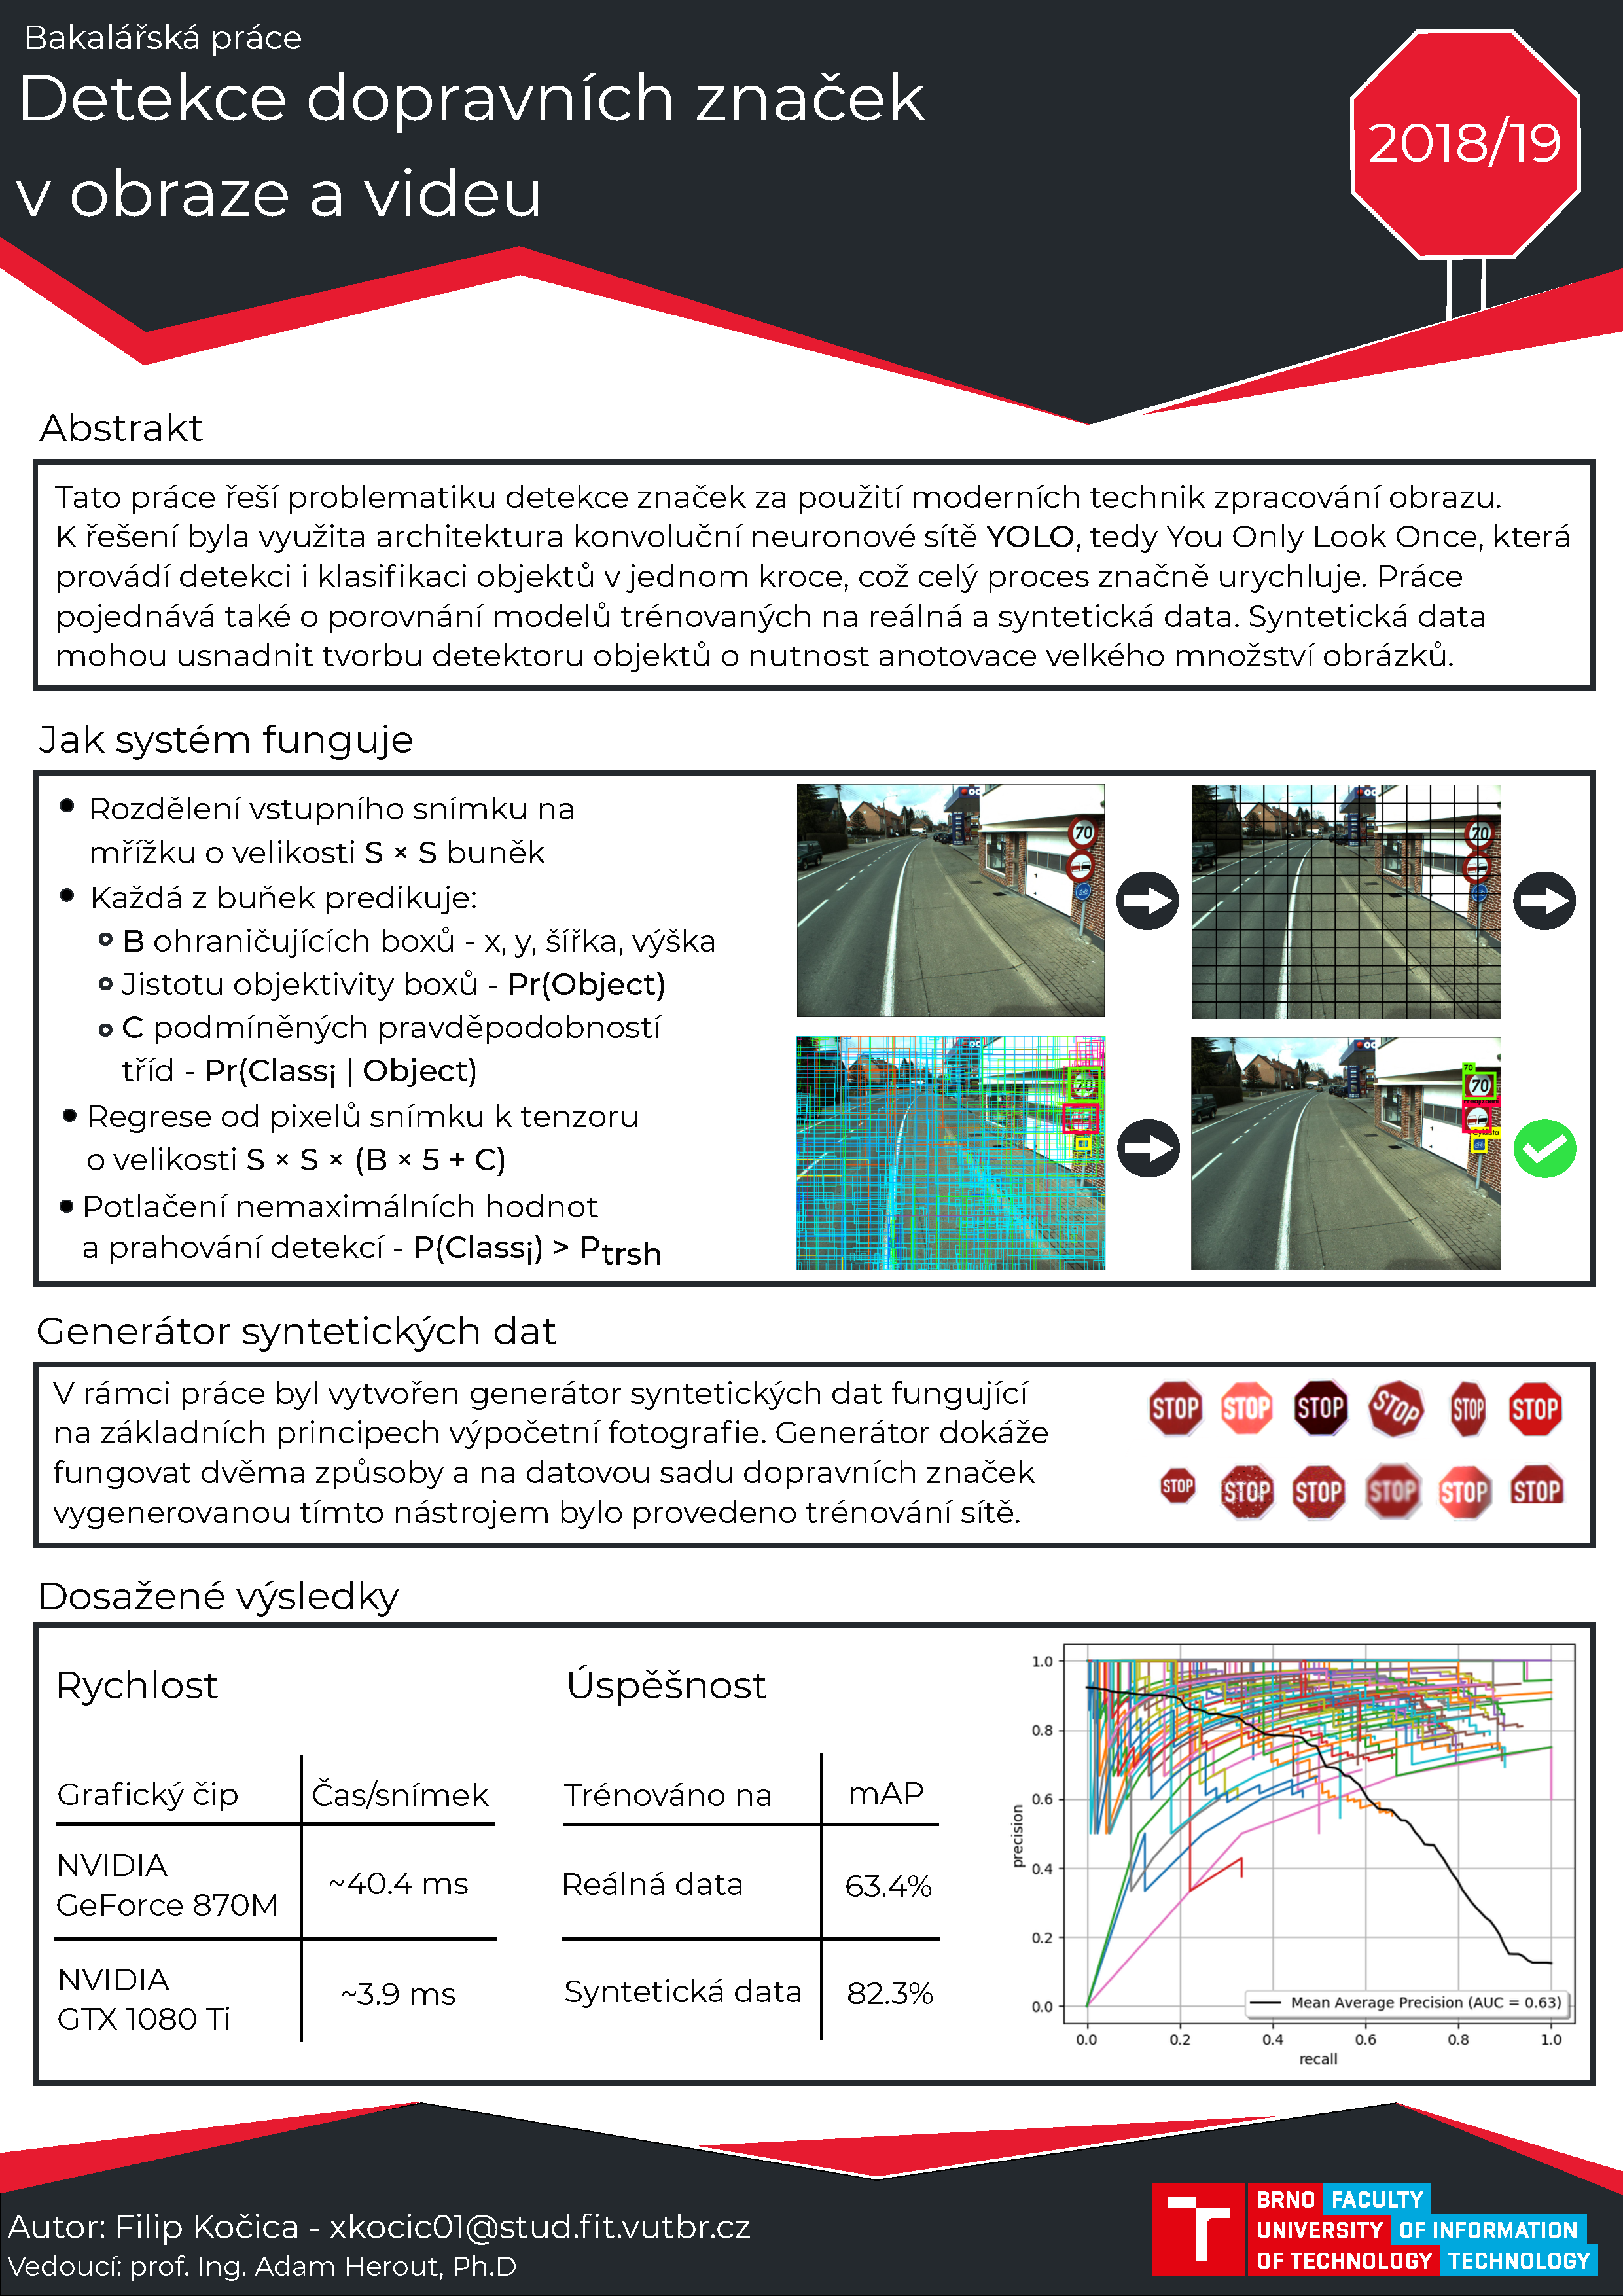
\includegraphics[width=0.75\linewidth]{figures/prilohy/poster.pdf}
\end{center}